\section{Desenvolvimento}
	Nesta seção, vamos mostrar e explicar os artefatos utilizados no processo de 
	design (produção) da interface a partir dos modelos de interação.
	\subsection{Da Interação Para o Design}
		Para poder realizar o design de interface para um sistema computacional, é necessário que hajam cenários 
		de interação nos quais se basear. Isto é, não se pode produzir uma interface 
		sem que se saiba de antemão os objetivos e funções que o sistema deverá oferecer.
		
		Por esse motivo, nosso trabalho foi baseado em Modelos de Mnteração, os 
		quais por sua vez são baseados em Cenários de Interação. Cenários de Interação 
		são descrições brevemente detalhadas sobre as ações do usuário e as respectivas
		respostas do sistema necessárias para o usuário alcançar seus objetivos \cite{ihc:barsil}. 
		Modelos de Interação são baseados em cenários de interação, e são constituídos 
		pelas conversas que o usuário vai ter com o sistema durante sua utilização.
		
		A modelagem que seguimos foi a que está disponível em \cite{ihc:barsil}. Ela 
		é formulada na linguagem de modelagem MoLIC\footnote{Modeling Language for Interacion 
		as Conversation}. MoLiC é uma linguagem para a modelagem da interação humano-computador
		como uma conversa, que as constrói em formato de diagramas de fluxo. A 
		elaboração de modelos dessa ordem é um passo anterior 
		ao design de interface, assim por esse motivo não estaremos explicando como 
		são elaborados tais modelos.
		
		O diagrama MoLIC em que o design foi baseado é um modelo de sistema de apoio 
		ao professor, sendo que este deverá poder lançar avisos aos alunos, disponibilizar 
		materiais e avaliar atividades enviadas pelos alunos. A figura seguinte ilustra 
		o próprio diagrama:
		
		\begin{figure}[!ht]
			\centering
			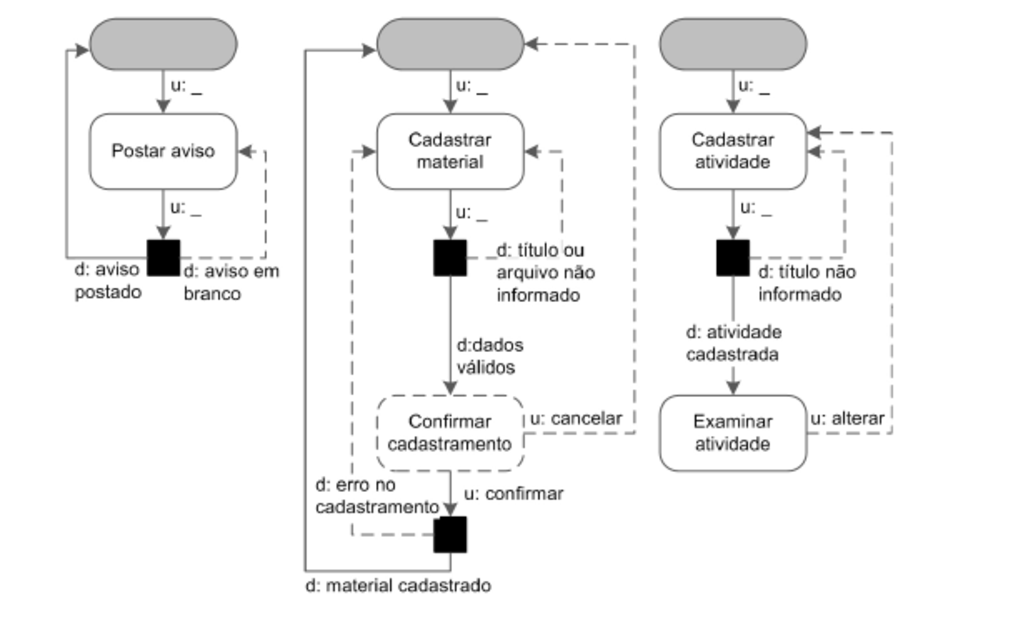
\includegraphics[scale=0.7]{molic.pdf}
			\caption{Diagrama MoLIC em que a interface foi baseada}
		\end{figure}
		
	\subsection{Design de Interface}
	
		\subsubsection{Estilos de Interação}
			Prude está fazendo.
		
		\subsubsection{Criação das Interfaces}
			A partir dos diagramas MoLIC, e das definições dos estilos de interação, 
			foram desenvolvidas os \emph{wireframes} das interfaces. Para tanto, utiliza-mo-nos
			do software \emph{web-based} chamado \emph{mockingbird}\footnote{https://gomockingbird.com/}.
			
			Como o sistema a ser desenvolvido requer portabilidade, nossa 
			interface segue o padrão de págnas da internet. Assim, temos uma página 
			inicial (que a princípio não estava proposta no modelo de interação, mas fez-se
			necessária) que oferece acessos ubíquos aos demais recursos do sistema, e que 
			pode ser usada para exibição de outras informações pertinentes -- funcionalidade essa que, devido ao 
			tempo restrito para elaboração do design, não foi implementada.
			
		
			Na sequencia, o \emph{wireframe} criado foi a interface para a unidade de 
			apresentação \texttt{Avisos}, também não especificado pela modelagem, mas que foi 
			entendido como ferramenta indispensável ao sistema, e que segue uma prototipação
			muito semelhante à da unidade de apresentação \texttt{Materiais}. Nela encontramos 
			Uma lista com os avisos já disponibilizados 
			pelo professor e um link \texttt{Adicionar Novo Aviso}.
		
		
		
		
		
		
		
		
		
		
		
		
		
		
		
		
		
		
		
